\documentclass[prb,preprint]{revtex4-1} 

\usepackage{amsmath}
\usepackage{amsfonts}
\usepackage{graphicx}

\begin{document}

\title{A Verification of the Fundamental Charge \\ Using Millikan's Oil Drop Experiment}

\author{Ryan S. Morshead}

\affiliation{Department of Physics, California State Polytechnic University...}

\date{October 23, 2013}

\begin{abstract}
Lightweight oil is sprayed through an atomizer. As the droplets are forced through the nozzle they gain a small amount of charge due to friction. The drops will quickly reach terminal velocity in the absence of any electric field and will travel at a constant velocity. By placing the drops between two electrodes, the electric field created by a voltage on them will cause the droplets to accelerate up and down. However. they will still rapidly achieve a terminal velocity. After measuring the terminal velocities of the drops under different, but known electric fields, the fundamental unit of charge $(e)$ can be calculated. That charge, reported here to be in agreement with the known value, is $1.570\pm0.045\times10^{-19}$.
\end{abstract}


\maketitle


\section{Introduction}

With the discovery of charged subatomic particles in the early 20th century by J.J. Thomson in 1897 and Neils Bohr, whose combined theories began to describe the internal workings of the atom, there was the question of how much charge these particles carried. At the time Robert A. Millikan, with significant input from Harvey Fletcher, perfected their oil drop experiment to measure the charge on one of the known sub atomic particles, the electron. The experiment involved measuring the force on oil droplets in a glass chamber sandwiched between two electrodes, one above and one below. With the electrical field calculated, one could measure the droplet's charge. The straightforward nature of the measurements and the conclusions that could be drawn from them became a foundation for Bohr's model of the atom, and the work that would eventually become the standard model. It convinced even the most stubborn skeptics; prior to Millikan's work Thomas Edison strongly believed that electric charge existed on an unbroken continuum, however after he spent some time working with Millikan, examining the method and results of the experiment he was swayed from his position. In the end Millikan's measurement of the fundamental charge was exceptional, and the method of measurement was an elegant hands on representation of the quantized world of atoms. 

The work done in this experiment looks to measure the fundamental charge as Millikan did by manipulating charged oil drops with electric fields.

\newpage

\section{Experimental Design}
Using an atomizer filled with low vapor pressure oil, small drops of oil are produced that carry a minute charge as a result of the friction endured while exiting the nozzle of the atomizer. The oil drops are introduced into a sub-chamber above the primary one depicted in Fig. \ref{ExpFig}. The drops are allowed to pass through a small closable vent in the top of the primary chamber into a cavity. Above and below the cavity are electrodes which can be used to manipulate the movements of the charged droplets when voltage is applied to them. Then using a light source on the end of the primary chamber opposite the viewing telescope the oil droplets are backlit with a lamp for easy viewing. The low vapor pressure of the oil ensures that the mass and volume of the drops will stay relatively constant throughout the measurement procedure -- most liquid compounds would evaporate in the presence of a heat source like the backlight.

\begin{figure}[h]
\centering
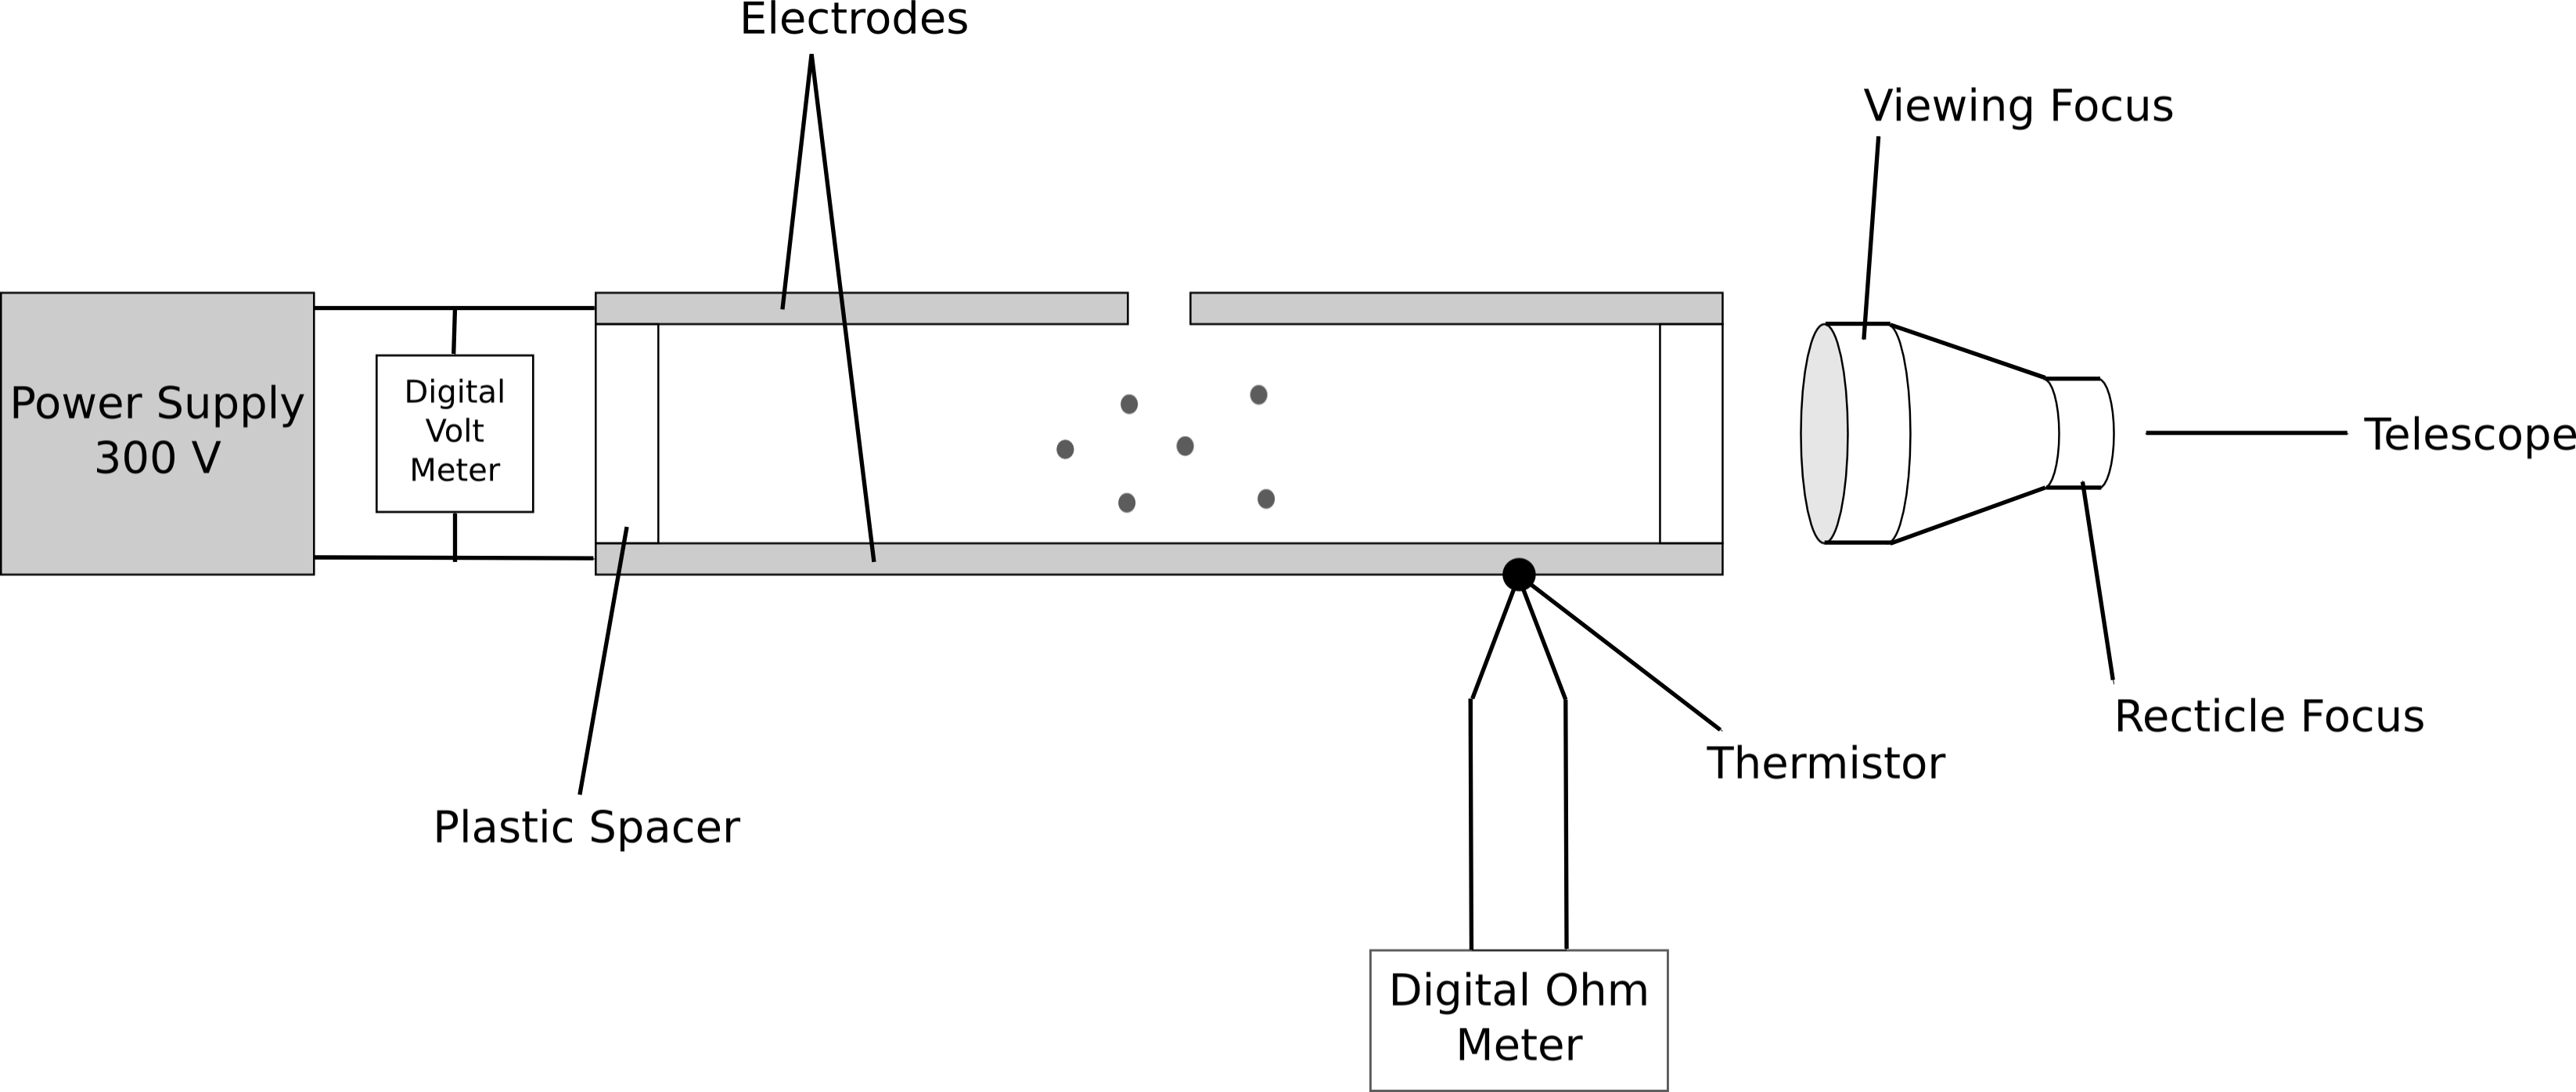
\includegraphics[width=\textwidth]{ExpFig.png}
\caption{Values of q on each drop with falling and forced fall values}
\label{ExpFig}
\end{figure}

Calipers are used to measure the thickness of the plastic separator and thus the electrode separation $d$. A voltmeter is then used to determine the voltage $V$ on the electrodes. With $d$ and $V$ being known quantities, Equation \eqref{Efield} is used to find the strength of the electric field generated by the electrodes.

\begin{equation}\label{Efield}
E = \frac{V}d.
\end{equation}

The grid found in the viewing scope is used to quantify distances inside the primary chamber by providing a fixed reference point. With measurements of distance in the chamber and a timer the velocity of the oil drops in the chamber can be calculated. By controlling the direction of the electric field in the chamber (either up, down, or neutral) the droplets are accelerated to their terminal velocities in milliseconds. In order to work back to the charge that induces the forces experienced by particles in different electric fields, the terminal velocity without the influence of electric fields $v_f$ and the radius $r$ of a spherical object moving slowly through a homogeneous medium of constant density must be related with Stokes Law in Equation \eqref{Stokes}.

\begin{equation}
\label{Stokes}
v_f = \frac{2 g \rho r^2}{9 \eta}.
\end{equation}

Using the thermistor shown in Fig. \ref{ExpFig} a temperature dependent resistance is then measured. A calibration curve developed with data points of known temperature and resistance can be used to correlate resistance read outs to particular temperatures. With this, the viscosity of the medium $\eta$ found in Equation \eqref{Stokes}, can be determined using Equation \eqref{eta}

\begin{equation}\label{eta}
\eta = \left (1.800 + \frac{T(in ^oC) - 15.0 ^oC}{209} \right ) \cdot 10^{-5}.
\end{equation}

By knowing the density of the oil used and the values determined by the previous calculations, algebraic manipulation of Equation \eqref{Stokes} will yield the radius of the spherical object  which is passing through the medium. Then, by applying the radius and density of the drop to the spherical mass formula in Equation \eqref{mass} the mass of the drop can be determined.

\begin{equation}\label{mass}
m=\frac{4}{3} \pi r^3 \rho.
\end{equation}

With $g$ being a known constant and $v_f$, $m$, and $E$ calculated, an analysis of the net force acting on the particle to maintain a terminal velocity in the presence of an electric field will yield equations \eqref{qu}, \eqref{qd}.

\begin{equation}\label{qu}
q_u = \frac{mg}{E}\left(\frac{v_u}{v_f}+1\right),
\end{equation}

\begin{equation}\label{qd}
q_d=\frac{mg}{E}\left(\frac{v_d}{v_f}-1\right),
\end{equation}

Where $v_u$ is the terminal speed of the drop under an electric field that induces an upwards pointing force while $v_d$ is the terminal speed of the particle while forced downwards by the reversed field.

This would appear to be the final step. However, at this point the calculations would lead one to believe that the charge of the particle is slightly dependent on the size of the drop. This is caused by a failure in the assumptions made in Stokes Law. Due to the tiny radii of the drops, the medium cannot be considered homogeneous and must instead be taken to be more granular. Thus a clever correction factor devised by Millikan can account for this. Equation \eqref{correct}, the correction factor shown below, is then simply multiplied to the calculated charge to compensate for the assumptions made in stokes law.

\begin{equation}\label{correct}
\gamma = \left (\frac{1}{1+b/r}\right)^{3/2} .
\end{equation}

\section{Analysis and Results}

Following the measurement of the charge on each valid oil drop (drops which had measurable $v_u$'s, $v_d$'s, and $v_f$'s) they were compared to the accepted value of $e$. In order to determine whether the values of $q$ corresponded to a fundamental charge, an appropriate integer divisor $n$ was found for each $q$ which could most accurately make values of $q/n$ converge to a single number. This value, to which all measurements of $q$ are integer multiples, is the fundamental charge reported by this paper. The results for the charge on each drop are shown in Fig. \ref{Graph}. The $q$ values as well as their associated integer multiples, evaluations of $e$ $(q/n)$, and errors are displayed in Table \ref{Trials}.

It should be noted that within each trial a single drop is treated as two. This is due to the fact that between measurements the charge of the drop may not, and in all our measurements, did not remain constant. As such, the variability of $q$ between measurements requires that the drops be treated as unique.



\begin{figure}[h!]
\centering
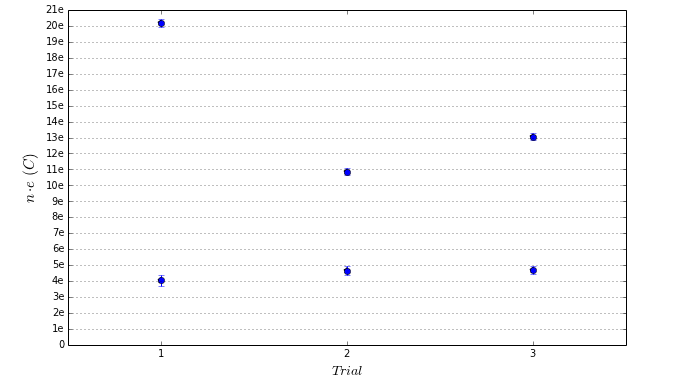
\includegraphics[width=\textwidth]{OilGraph.png}
\caption{Measured charges on oil drops based on $v_u$ and $v_d$ as compared to the integer multiples of the accepted value $e$.}
\label{Graph}
\end{figure}


\begin{table}[h!]
\centering
\caption{Trials and their corresponding values and uncertainties.}
\begin{ruledtabular}
\begin{tabular}{c c c c c c p{4 cm}}
Drop Number&$q$ (C)&$\delta q$ (C)&$n$& $e=q/n$ $(C)$ &$\delta e=\delta q /n$ (C)\\
\hline
1 &3.2339x$10^{-18}$& 4.11x$10^{-20}$&20&1.617x$10^{-19}$&2.1x$10^{-21}$\\
2& 1.7386x$10^{-18}$&3.74x$10^{-20}$&11&1.581x$10^{-19}$&3.4x$10^{-21}$\\
3&2.0909x$10^{-18}$&3.48x$10^{-20}$&13&1.608x$10^{-19}$&2.7x$10^{-21}$\\
4&6.4678x$10^{-19}$&5.78x$10^{-20}$&4&1.617x$10^{-19}$&1.4x$10^{-20}$\\
5&7.4586x$10^{-19}$&4.40x$10^{-20}$&5&1.492x$10^{-19}$&8.8x$10^{-21}$\\
6&7.4914x$10^{-19}$&4.13x$10^{-20}$&5&1.498x$10^{-19}$&8.3x$10^{-21}$\\
\end{tabular}
\end{ruledtabular}
\label{Trials}
\end{table}



\newpage
All the results for the values of $q/n$ shown in Table \ref{Trials} are in agreement with the accepted value of $1.602\times10^{-19}$ C. The average, $1.570\pm0.045\times10^{-19}$ C, of these values, though not better approximations of $e$ than some of the individual measurements, still can be said to be in agreement with accepted value for $e$.

\section{Conclusion}

The purpose of this experiment was to confirm the accepted value of the fundamental unit of charge by measuring the charge on oil droplets forced through an atomizer by subjecting them to electric fields in the manner devised by Robert Millikan in the early 20$^{th}$ century. This goal was achieved, as all the results from Table \ref{Trials} and the average of those results, $1.570\pm0.045\times10^{-19}$ C, agree with the accepted value.

\newpage

\begin{acknowledgments}

We're supposed to govern the clock, not be governed by it. But when do we have time to do even that?

\end{acknowledgments}


\begin{thebibliography}{99}l.

\end{thebibliography}

\end{document}
